% !TEX program = pdflatex
% First-version design, refined: sequential numbering, larger type, fuller layouts.
\documentclass[12pt,aspectratio=169,xcolor={dvipsnames,table}]{beamer}
\geometry{paperwidth=240mm,paperheight=135mm}
\usetheme{KhNU}
\usepackage[T1]{fontenc}
\usepackage[utf8]{inputenc}
\usepackage{amsmath,amssymb,booktabs,tabularx,array,graphicx,makecell,textcomp}
\usepackage{lmodern}\renewcommand{\sfdefault}{phv}
\usefonttheme{professionalfonts}
\usetikzlibrary{calc,positioning,arrows.meta}
\renewcommand{\normalsize}{\fontsize{14.5}{17}\selectfont}
\renewcommand{\small}{\fontsize{12.4}{14.6}\selectfont}
\renewcommand{\footnotesize}{\fontsize{11.5}{13.5}\selectfont}
\renewcommand{\scriptsize}{\fontsize{10.5}{12.2}\selectfont}
\renewcommand{\large}{\fontsize{17}{20}\selectfont}
\renewcommand{\Large}{\fontsize{21.5}{25}\selectfont}
\renewcommand{\LARGE}{\fontsize{25.5}{30}\selectfont}
\definecolor{ink}{HTML}{142F49}
\definecolor{teal}{HTML}{087F8C}
\definecolor{muted}{HTML}{546A7C}
\definecolor{bluewash}{HTML}{EEF5FA}\definecolor{blueink}{HTML}{245884}
\definecolor{greenwash}{HTML}{E7F3EC}\definecolor{greenink}{HTML}{276449}
\definecolor{amberwash}{HTML}{FFF2DF}\definecolor{amberink}{HTML}{78521E}
\definecolor{rosewash}{HTML}{F8EBE9}\definecolor{roseink}{HTML}{833F40}
\setbeamercolor{normal text}{fg=ink,bg=white}
\setbeamercolor{frametitle}{fg=ink}
\setbeamercolor{card blue}{fg=ink,bg=bluewash}
\setbeamercolor{card green}{fg=ink,bg=greenwash}
\setbeamercolor{card amber}{fg=ink,bg=amberwash}
\setbeamercolor{card rose}{fg=ink,bg=rosewash}
\setbeamercolor{signal}{fg=white,bg=teal}
\setbeamersize{text margin left=9mm,text margin right=9mm}
\setbeamertemplate{navigation symbols}{}
\setbeamertemplate{background}{}\usebackgroundtemplate{}
\setbeamertemplate{frametitle}{%
\vspace{1mm}\begin{minipage}[c][11mm][c]{.88\linewidth}
{\Large\bfseries\insertframetitle\par}\end{minipage}\hfill
\begin{minipage}[c]{17mm}\centering
\includegraphics[height=12mm,width=16mm,keepaspectratio]{logos/logo_adt-ismddc.png}\end{minipage}\par
{\color{teal}\rule{\linewidth}{.6pt}}\vspace{-.5mm}}
\setbeamertemplate{footline}{%
\hspace*{9mm}\begin{minipage}{222mm}
{\color{dexpiLightBlue}\rule{\linewidth}{.4pt}}\par
\vspace{1mm}{\scriptsize\color{muted}Radiuk, Barmak \& Krak\hfill\insertsection\hfill\insertframenumber\,/\,\inserttotalframenumber\par}
\vspace{2mm}\end{minipage}}
\setlength{\tabcolsep}{3pt}\renewcommand{\arraystretch}{1.03}
\newcolumntype{Y}{>{\raggedright\arraybackslash}X}
\newcolumntype{C}{>{\centering\arraybackslash}X}
\setlength{\abovedisplayskip}{3pt}\setlength{\belowdisplayskip}{3pt}
\hypersetup{colorlinks=true,urlcolor=teal,linkcolor=teal,
pdftitle={Auditing Deep Learning for Cardiac MRI Through Semantic Transitions and Conflict-Aware Production Rules},
pdfauthor={Pavlo Radiuk; Oleksander Barmak; Iurii Krak}}
\newcommand{\matA}{\mathbf A}\newcommand{\matB}{\mathbf B}
\newcommand{\matT}{\mathbf T}
\DeclareMathOperator*{\argmin}{arg\,min}\newcounter{auditalgorithm}
\newcommand{\captext}[1]{{\scriptsize\color{muted}#1\par}}
\newcommand{\kicker}[1]{{\small\bfseries\color{teal}#1\par}\vspace{1.5mm}}
\newcommand{\takeaway}[1]{\par\noindent\begin{beamercolorbox}[wd=\dimexpr\linewidth-3pt\relax,sep=2.2mm]{signal}{\small\bfseries #1\par}\end{beamercolorbox}\par}
\newcommand{\card}[3][blue]{\par\noindent\begin{beamercolorbox}[wd=\dimexpr\linewidth-3pt\relax,sep=3mm]{card #1}
{\small\bfseries\color{#1ink}#2\par}\vspace{1.5mm}{\small #3\par}\end{beamercolorbox}\par}
% Counters advance only in presentation order. Source label keys remain semantic.
\newcommand{\tbl}[2]{\refstepcounter{table}\kicker{Table \thetable. #2}{\footnotesize\input{content/table-#1.tex}\par}}
\newcommand{\figurecap}[2]{\refstepcounter{figure}\label{#1}\captext{\textbf{Figure \thefigure.} #2}}
\newcommand{\mathsize}{\fontsize{13.2}{15.6}\selectfont}
\newcommand{\eqn}[1]{{\mathsize\input{content/equation-#1.tex}}}

\newcommand{\scorebar}[2]{#1\hspace{1mm}\begin{tikzpicture}[x=1mm,y=1mm,baseline=0]
\fill[muted!12] (0,0) rectangle (22,2.8);\fill[#2] (0,0) rectangle (22*#1,2.8);\end{tikzpicture}}
\begin{document}

% 1. Retain the first version's navy title and angular blue accent.
\begin{frame}[plain]
\small
\begin{tikzpicture}[remember picture,overlay]
\fill[ink] (current page.north west) rectangle ([yshift=-75mm]current page.north east);
\fill[dexpiBlue] ([xshift=-53mm]current page.north east)--(current page.north east)--([yshift=-75mm]current page.north east)--([xshift=-75mm,yshift=-75mm]current page.north east)--cycle;
\draw[teal,line width=3pt] ([xshift=9mm,yshift=-77mm]current page.north west)--([xshift=78mm,yshift=-77mm]current page.north west);
\node[anchor=north west,text width=211mm,inner sep=0pt,text=white] at ([xshift=9mm,yshift=-10mm]current page.north west) {\small CMR SEMANTICS\quad/\quad EXPLAINABLE AI\quad/\quad SELECTIVE AUDITING};
\node[anchor=north west,text width=211mm,inner sep=0pt,text=white] at ([xshift=9mm,yshift=-24mm]current page.north west) {\LARGE\bfseries Auditing Deep Learning for Cardiac MRI\\[1mm]Through Semantic Transitions and\\[1mm]Conflict-Aware Production Rules};
\node[anchor=north west,text width=211mm,inner sep=0pt,text=white] at ([xshift=9mm,yshift=-64mm]current page.north west) {\small Cardiac magnetic resonance (CMR): measurable semantics and guarded rules};
\node[anchor=north west,text width=211mm,inner sep=0pt,text=ink] at ([xshift=9mm,yshift=-85mm]current page.north west) {\normalsize\bfseries Pavlo Radiuk\textsuperscript{1}\quad Oleksander Barmak\textsuperscript{1}\quad Iurii Krak\textsuperscript{2,3}};
\node[anchor=north west,text width=211mm,inner sep=0pt,text=ink] at ([xshift=9mm,yshift=-96mm]current page.north west) {\small\textsuperscript{1}Khmelnytskyi National University\\[1mm]\textsuperscript{2}Taras Shevchenko National University of Kyiv\\[1mm]\textsuperscript{3}V.M. Glushkov Institute of Cybernetics};
\node[anchor=north west,text width=211mm,inner sep=0pt,text=muted] at ([xshift=9mm,yshift=-122mm]current page.north west) {\scriptsize ADT-ISMDDC @ ICST-ODESA\quad |\quad September 22--24, 2026};
\end{tikzpicture}
\end{frame}

\section{Relevance}
% 2. Tables 1–2, both enlarged and transposed.
\begin{frame}[t]{Prediction quality leaves an audit gap}
\small
\begin{columns}[T,onlytextwidth]
\column{.49\textwidth}\tbl{1}{Accuracy and absolute error}
\vspace{1mm}\card{The audit gap}{Link recognizable measurements to rules, provenance, conflict, and safe abstention.}
\column{.49\textwidth}\tbl{2}{Correlation, bias, and audit outputs}
\end{columns}
\vspace{2mm}\captext{Table 2: Pearson $r$ and signed bias. pp = percentage points. Study: transition + semantic baseline / rule audit.\\Table highlights: \textcolor{blueink}{\textbf{blue:}} reported result; \textcolor{amberink}{\textbf{amber:}} guarded abstention; \textcolor{roseink}{\textbf{rose:}} error / drift flag; \textcolor{greenink}{\textbf{green:}} proxy evidence.}
\vspace{1mm}\takeaway{Different splits and objectives: context, not a controlled ranking.}
\vspace{1mm}\captext{O. Bernard et al. ``Deep Learning Techniques for Automatic MRI Cardiac Multi-Structures Segmentation and Diagnosis: Is the Problem Solved?'' \textit{IEEE Transactions on Medical Imaging}, 37(11):2514--2525, 2018. \href{https://doi.org/10.1109/TMI.2018.2837502}{doi:10.1109/TMI.2018.2837502}.}
\end{frame}

\section{Purpose and objectives}
% 3. Table 3 and a balanced three-card layout.
\begin{frame}[t]{Make every audit output traceable}
\small
\takeaway{Purpose: translate fixed CMR representations into measurable semantics and guarded rules.}
\vspace{3mm}\begin{columns}[T,onlytextwidth]
\column{.32\textwidth}\card{01 / Align}{Patient identity, feature QC, and source provenance.}
\column{.32\textwidth}\card[green]{02 / Reconstruct}{128 formal coordinates $\rightarrow$ 28 CMR measurements.}
\column{.32\textwidth}\card[amber]{03 / Audit}{Rule support, conflict, missing evidence, and abstention.}
\end{columns}
\vspace{2mm}\captext{ACDC = Automated Cardiac Diagnosis Challenge.\\M\&Ms = Multi-Centre, Multi-Vendor and Multi-Disease Cardiac Segmentation.}
\vspace{2mm}\tbl{3}{Cohorts and release-level quality control}
\vspace{2mm}\captext{\textcolor{roseink}{\textbf{QC (quality control):}} 92 pending reviews across both cohorts; not confirmed errors or completed expert validation.}
\end{frame}

\section{Methods}
% 4. Original manuscript architecture, alongside a compact audit summary.
\begin{frame}[t]{A frozen, patient-level audit chain}
\small
\begin{columns}[T,onlytextwidth]
\column{.76\textwidth}
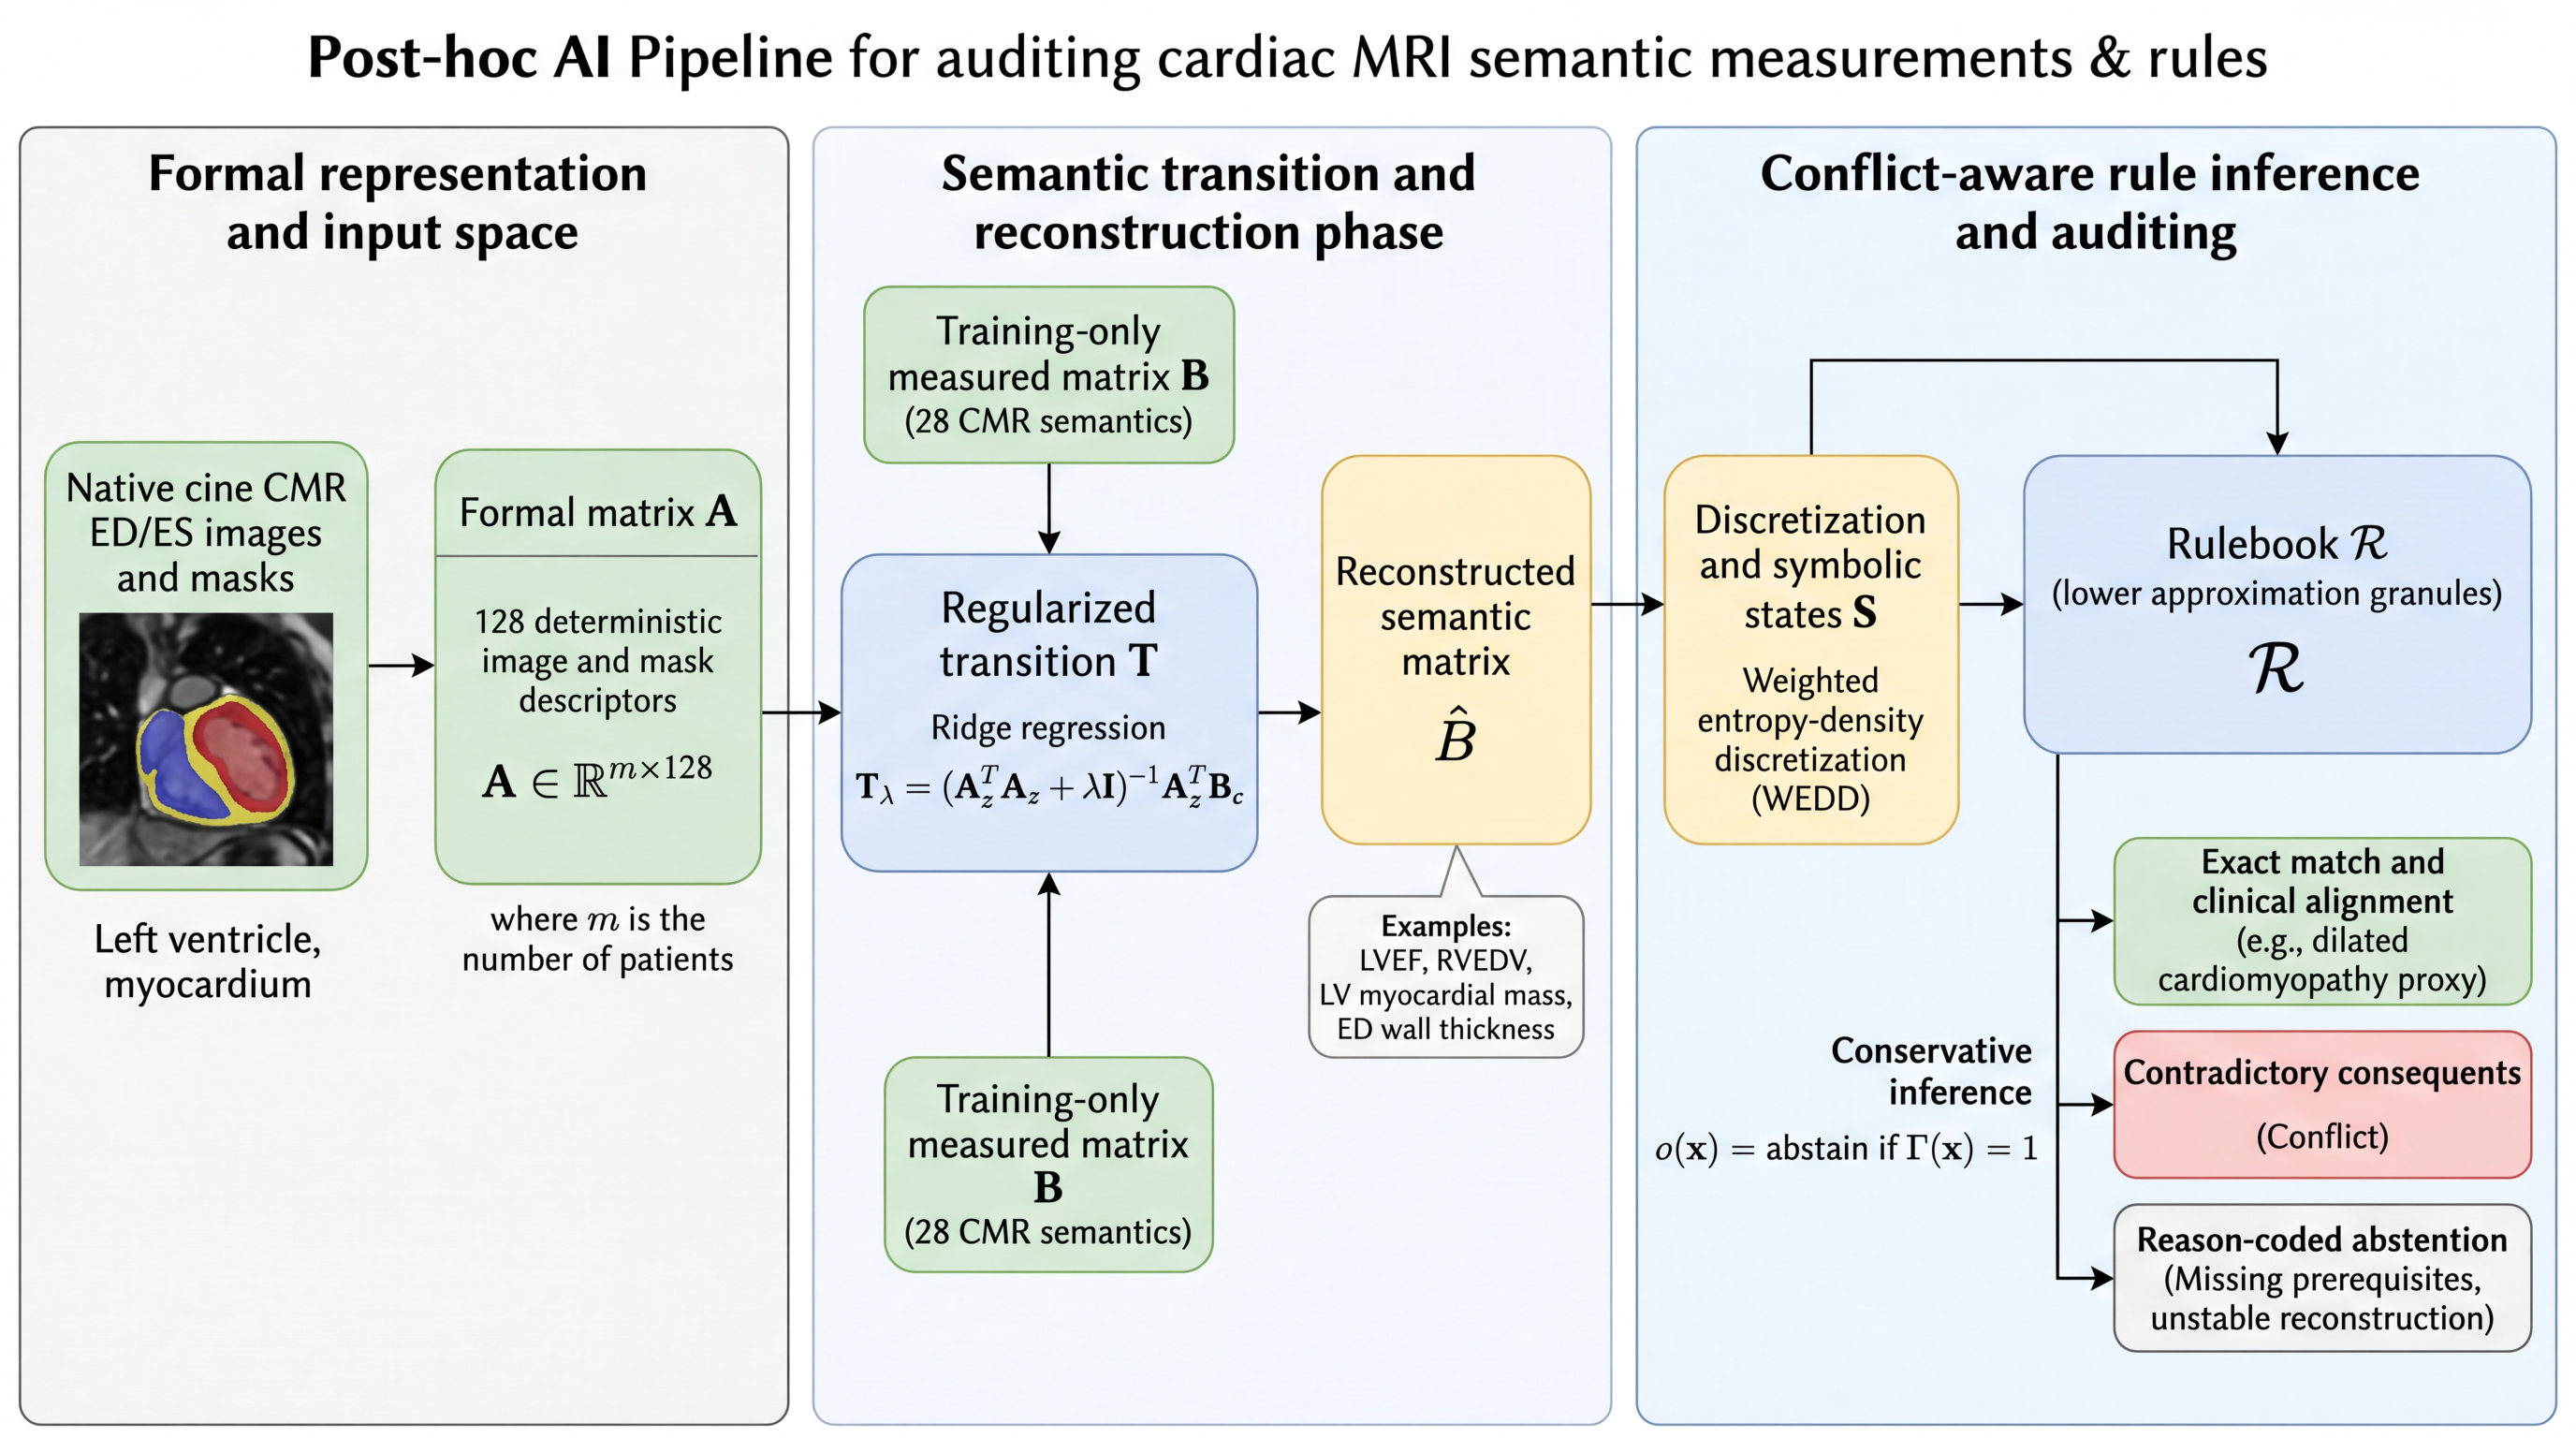
\includegraphics[width=\linewidth,trim=0 0 0 50bp,clip]{figures/fig_audit-architecture.pdf}\par
\vspace{1mm}\figurecap{fig:cmr_audit_architecture}{Framework architecture; the evaluated release substitutes training tertiles for the weighted entropy-density discretization (WEDD) block.}
\column{.22\textwidth}
\refstepcounter{auditalgorithm}\label{alg:cmr_audit_pipeline}
\card{Algorithm 1}{\footnotesize
1. Lock cohorts + QC\\[1mm]
2. Fit transition\\[1mm]
3. Discretize\\[1mm]
4. Induce rules\\[1mm]
5. Guard inference\\[1mm]
6. Align predicates\\[1mm]
7. Evaluate fidelity\\[1mm]
8. Test perturbations}
\vspace{3mm}\card[amber]{Evaluated release}{\footnotesize
57 descriptors projected to 128 coordinates.\\[2mm]
The WEDD block is approximated by frozen training tertiles.}
\end{columns}
\end{frame}

% 5. Enlarged equations and cards occupy the former blank space.
\begin{frame}[t]{Regularized semantic reconstruction}
\small
\begin{columns}[T,onlytextwidth]
\column{.57\textwidth}\card{Ridge fit and frozen reconstruction}{\eqn{1}\eqn{2}\eqn{3}}
\vspace{4mm}\card[amber]{Training-only preprocessing}{Median imputation; 1st--99th percentile clipping; formal standardization; target centering. Five-fold training cross-validation selected $\lambda$ = 3.}
\column{.40\textwidth}\card[green]{Evaluated representation}{57 deterministic descriptors $\rightarrow$ 128 coordinates by a fixed Gaussian projection; 32 direct channels retained. Seed: 20260611.}
\vspace{4mm}\card{Frozen tertile states}{\noindent\begin{minipage}{\dimexpr\linewidth-6mm\relax}\eqn{4}\end{minipage}}
\end{columns}
\vspace{4mm}\captext{$\mathbf A_z$: standardized formal features; $\mathbf B_c$: centered targets; $\boldsymbol\mu_B$: training means. The 28 targets cover volumes, EF, mass, wall thickness, and shape.}
\vspace{3mm}\takeaway{This experiment uses deterministic descriptors and tertiles; transition coefficients express associations.}
\end{frame}

% 6. Math typeset at readable sizes; Equation 7 wraps instead of shrinking.
\begin{frame}[t]{Rules, guards, and clinical alignment}
\small
\begin{columns}[T,onlytextwidth]
\column{.49\textwidth}\card{Compact production rules}{\eqn{5}\textbf{At most 3 antecedents}; support at least 3 cases; confidence at least 0.60.}
\vspace{3mm}\card[amber]{Guarded inference}{\eqn{6}}
\vspace{2mm}\captext{$\Gamma(x)$: guard; $\rho(x)$: reason code; $\mathcal Y(x)$: fired consequents. Guards cover severe QC, unstable reconstruction, missing prerequisites, no match, and contradictory consequents.}
\column{.49\textwidth}\card[green]{Physician-style alignment}{\eqn{7}}
\vspace{2mm}\captext{$\phi_j$: compatibility; $w_j$: clinical weights. $C_i,M_i,U_i,A_i$: conflict, missing evidence, instability, and safe abstention.}
\vspace{3mm}\card[rose]{Eligibility before similarity}{Only rules passing support, confidence, prerequisite, and validity gates are eligible.}
\end{columns}
\vspace{2mm}\takeaway{Soft similarity never overrides the abstention guard. Cine-supported proxies remain evidence-bounded.}
\end{frame}

\section{Experiments and results}
% 7. Tables 4–5, Figures 2–3; enlarged data and chart labels.
\begin{frame}[t]{Semantic fidelity and external domain shift}
\small
\begin{columns}[T,onlytextwidth]
\column{.38\textwidth}\tbl{4}{Aggregate reconstruction}
{\eqn{8}}
\captext{NRMSE: normalized root mean square error (training SD); SD: standard deviation. MAE: mean absolute error.}
\vspace{1mm}\centering\begin{tikzpicture}[x=1mm,y=.22mm]
\foreach \y in {0,50,100} {
 \draw[muted!22] (0,\y)--(72,\y);
 \node[font=\scriptsize,anchor=east,text=muted] at (-1,\y) {\y};
}
\foreach \x/\a/\b/\lab in {8/33.18/26.49/Train,26/58.42/46.49/Val.,44/51.65/38.64/Test,62/85.35/69.81/Ext.} {
 \fill[dexpiBlue] (\x-3,0) rectangle (\x,\a);
 \fill[amberink!75] (\x+1,0) rectangle (\x+4,\b);
 \node[font=\scriptsize,anchor=north,text=ink] at (\x+.5,-5) {\lab};
}
\end{tikzpicture}
\par
\figurecap{fig:transition_split_errors}{\textcolor{dexpiBlue}{\textbf{RMSE}} / \textcolor{amberink}{\textbf{MAE}}. M\&Ms external bias: LVEDV \textminus136.0 mL; mass \textminus96.6 g.}
\column{.60\textwidth}\tbl{5}{Held-out ACDC target fidelity}
\vspace{2mm}\captext{$n$ = 50; 1,000-resample bias-corrected and accelerated (BCa) 95\% confidence intervals (CIs). ED: end-diastolic; pp: percentage points.}
\vspace{1mm}\centering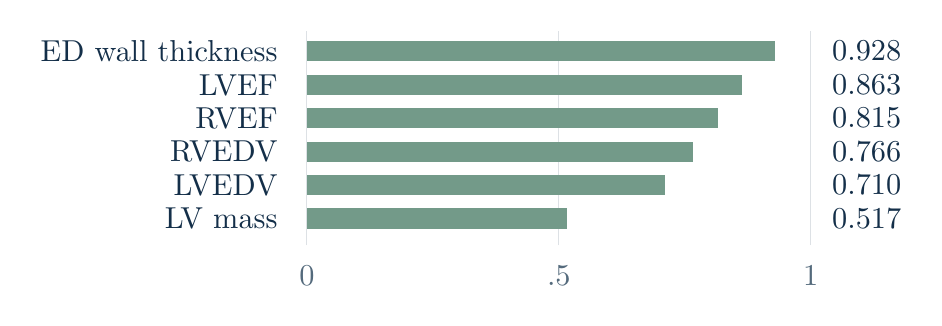
\begin{tikzpicture}[x=1mm,y=.85mm]
\foreach \x/\lab in {0/0,32/.5,64/1} {
 \draw[muted!20] (\x,0)--(\x,32);
 \node[font=\scriptsize,anchor=north,text=muted] at (\x,-1) {\lab};
}
\foreach \y/\v/\lab in {29/.928/ED wall thickness,24/.863/LVEF,19/.815/RVEF,14/.766/RVEDV,9/.710/LVEDV,4/.517/LV mass} {
 \node[font=\scriptsize,anchor=east,text=ink] at (-2,\y) {\lab};
 \fill[greenink!65] (0,\y-1.5) rectangle (64*\v,\y+1.5);
 \node[font=\scriptsize,anchor=west,text=ink] at (65,\y) {\pgfmathprintnumber[fixed,precision=3,zerofill,assume math mode=true]{\v}};
}
\end{tikzpicture}
\par
\figurecap{fig:high_impact_correlations}{High-impact target correlations (Pearson $r$, scale 0--1).}
\end{columns}
\vspace{.5mm}\captext{\textbf{External NRMSE is 2.25 times the held-out test error.} Mixed-unit RMSE / MAE means are descriptive.}
\end{frame}

% 8. Tables 6–7 use the full slide width.
\begin{frame}[t]{Coverage must accompany rule accuracy}
\small
\tbl{6}{Measured-semantic logistic-regression comparator}
\vspace{1mm}\tbl{7}{200-rule audit; balanced accuracy and F1 use non-abstained cases}
\vspace{2mm}\begin{columns}[T,onlytextwidth]
\column{.50\textwidth}\centering\begin{tikzpicture}[x=.99mm,y=.92mm]
\foreach \x/\lab in {0/0,32/0.5,64/1} {
 \draw[muted!20] (\x,0)--(\x,27);
 \node[font=\scriptsize,anchor=north,text=ink] at (\x,-1) {\lab};
}
\node[font=\scriptsize,anchor=east,text=ink] at (-2,25) {Rule decisions};
\fill[dexpiBlue] (0,23) rectangle (40.96,27);
\fill[amberink!65] (40.96,23) rectangle (64,27);
\node[font=\scriptsize,text=white] at (20.48,25) {64\%};
\node[font=\scriptsize,text=white] at (52.48,25) {36\%};
\foreach \y/\val/\lab in {19/.644/Rule bal. acc.,13/.612/Rule macro-F1,7/.860/Classifier acc.,1/.973/Classifier AUROC} {
 \node[font=\scriptsize,anchor=east,text=ink] at (-2,\y) {\lab};
 \fill[dexpiBlue] (0,\y-1.3) rectangle (64*\val,\y+1.3);
 \node[font=\scriptsize,anchor=west,text=ink] at (65,\y) {\pgfmathprintnumber[fixed,precision=3,zerofill,assume math mode=true]{\val}};
}
\end{tikzpicture}
\par
\figurecap{fig:classifier_rulebook_outcomes}{Held-out outcomes: \textcolor{blueink}{32 covered}; \textcolor{amberink}{18 abstained}.}
\column{.48\textwidth}\card[green]{Held-out uncertainty / 95\% CIs}{\footnotesize
Accuracy: 0.860 [0.76, 0.94]\\
Balanced accuracy: 0.860 [0.75, 0.95]\\
Macro-F1: 0.861 [0.75, 0.94]\\
AUROC: 0.973 [0.947, 0.993]\\[1mm]
Row-bootstrap intervals; $n$ = 50.}
\end{columns}
\vspace{.5mm}\captext{AUROC: area under the receiver operating characteristic curve. ECE: expected calibration error (10 equal-mass bins). Conflict: covered cases; conf. seen: all cases during resolution. Perfect selective train/validation scores reflect over-specific granules.}
\end{frame}

% 9. Tables 8–9 and Figure 5, clearly ordered left to right.
\begin{frame}[t]{Predicate alignment and perturbation sensitivity}
\small
\begin{columns}[T,onlytextwidth]
\column{.53\textwidth}
\refstepcounter{figure}\label{fig:predicate_alignment_scores}%
\refstepcounter{table}%
\kicker{Table \thetable\ with embedded Figure \thefigure.\\Physician-predicate evidence}
{\footnotesize\label{tab:predicate_evidence_alignment}
\begin{tabularx}{\linewidth}{@{}Y>{\raggedright\arraybackslash}p{26mm}r@{}}
\toprule
\textbf{Predicate family} & \textbf{Evidence} & \textbf{Similarity}\\
\midrule
Abnormal RV / ARVC proxy & Cine + mask & \scorebar{0.9008}{greenink}\\
HCM proxy & Cine + mask & \scorebar{0.8564}{greenink}\\
MI remodeling proxy & Cine & \scorebar{0.8250}{greenink}\\
DCM proxy & Cine + mask & \scorebar{0.7858}{greenink}\\
Valvular volume review & Review proxy & \scorebar{0.7825}{greenink}\\
Congenital review & Approximation & \scorebar{0.6842}{greenink}\\
Conservative normal filter & Research filter & \scorebar{0.5462}{greenink}\\
Other families & Unsupported & \textcolor{dexpiRedDark}{Unmatched}\\
\bottomrule
\end{tabularx}
\par}
\vspace{1mm}\captext{Bars: admissible similarity on a common 0--1 scale.\\Unmatched: restrictive, noncompaction, inflammatory, infiltrative.}
\vspace{1mm}\captext{HCM / DCM: hypertrophic / dilated cardiomyopathy; MI: myocardial infarction; ARVC: arrhythmogenic right ventricular cardiomyopathy.}
\vspace{1mm}\noindent\begin{beamercolorbox}[wd=\dimexpr\linewidth-3pt\relax,sep=2mm]{card green}{\small\textbf{Research proxies:} support review, not diagnosis or clinician agreement.\par}\end{beamercolorbox}
\vspace{1mm}\captext{Native orientation; no rotation augmentation.}
\column{.45\textwidth}\tbl{9}{Perturbations: 12 cases, 48 runs}
\vspace{1mm}{\mathsize\begin{align}
\Delta_A(\tau)&=\frac{1}{|Q|}\!\sum_{x\in Q}\!\frac{\|\mathbf a(\tau x)-\mathbf a(x)\|_2}{\|\mathbf a(x)\|_2+\varepsilon}.
\tag{9}\label{eq:formal_perturbation_change}\\[1mm]
\Delta_B(\tau)&=\frac{1}{28|Q|}\sum_{x\in Q}\|\widehat{\mathbf b}(\tau x)-\widehat{\mathbf b}(x)\|_1.
\tag{10}\label{eq:semantic_perturbation_change}
\end{align}
}
\vspace{1mm}\card[rose]{Orientation sensitivity}{A 2\textdegree{} rotation produces the largest drift despite nearly preserved mask counts.}
\vspace{.5mm}\captext{$Q$: 12 cases; $\tau$: perturbation; $\varepsilon$: stabilizer. Mixed-unit semantic drift ranks sensitivity only.}
\end{columns}
\end{frame}

\section{Conclusions and contact}
% 10. Enlarge and balance concluding cards, contacts, and identity strip.
\begin{frame}[t]{Transparent auditing and next validation}
\small
\begin{columns}[T,onlytextwidth]
\column{.49\textwidth}\card[green]{What the study establishes}{A traceable semantic-to-rule audit chain; strong internal association for selected targets; visible external degradation, conflict, and abstention.}
\vspace{2mm}\card[amber]{What remains to be validated}{Frozen deep encoders; full WEDD; orientation normalization; vendor recalibration; completed expert QC and prospective clinician evaluation.}
\vspace{2mm}\card[rose]{Current scope}{Research auditing only: domain shift and sparse rules limit clinical use.}
\column{.48\textwidth}\card{Authors and correspondence}{\textbf{Pavlo Radiuk}\textsuperscript{1} (corresponding author)\\\href{mailto:radiukp@khmnu.edu.ua}{radiukp@khmnu.edu.ua}\\[3mm]
\textbf{Oleksander Barmak}\textsuperscript{1}\\\href{mailto:barmako@khmnu.edu.ua}{barmako@khmnu.edu.ua}\\[3mm]
\textbf{Iurii Krak}\textsuperscript{2,3}\\\href{mailto:iurii.krak@knu.ua}{iurii.krak@knu.ua}}
\vspace{3mm}\captext{\textsuperscript{1}Khmelnytskyi National University\\\textsuperscript{2}Taras Shevchenko National University of Kyiv\\\textsuperscript{3}V.M. Glushkov Institute of Cybernetics}
\vspace{3mm}\captext{Supporting organizations and conference identities}
\vspace{2mm}{\small
\includegraphics[height=9mm]{logos/logo_ceur.png}\hfill
\includegraphics[height=9mm]{logos/logo_cs.png}\hfill
\includegraphics[height=11mm]{logos/logo_icst.png}\hfill
\includegraphics[height=11mm]{logos/logo_khnu.png}\par}
\end{columns}

\end{frame}
\end{document}
